\section{Model}
A dynamical model of the system is derived, first by Newton's method and then by the energy method. The model is based on the conventions presented in the mechanical diagram in \autoref{fig:mechanicalDrawing} while excessive coordinates are defined in \autoref{fig:excessiveCoordinates}. The cart is constrained to the horizontal rail s.t. $y_c = 0$, that is, the cart only ever moves along the $x$-axis.

%\begin{figure}[H]
%  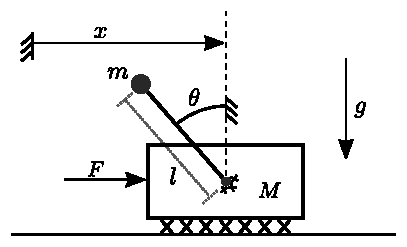
\includegraphics[width=.5\textwidth]{figures/mechanicalDrawing}
%  \caption{The cart pendulum system with generalized coordinates, $x$ and $\theta$, where $x$ is the center position of the cart, $\theta$ is the angle of the pendulum, $m$ is the point mass of the pendulum, $M$ is the mass of the cart, g is the gravitational acceleration and f is the force of actuation.}
%  \label{fig:mechanicalDrawing}
%\end{figure}

\begin{figure}[H]
  \hspace{-10pt}
  \captionbox
  {
    The cart pendulum system with excessive coordinates, where $(x_c, y_c)$ is the position of pendulum pivot point on the cart and $(x_p, y_p)$ is the position of the pendulum point mass.
    \label{fig:excessiveCoordinates}
  }
  {
    \hspace{-1cm}
    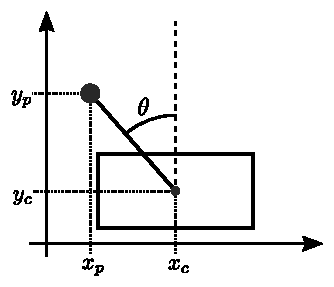
\includegraphics[width=.4\textwidth]{figures/excessiveCoordinates}\vspace{-11pt}
  }
  \hspace{20pt}
  \captionbox 
  {
    Mechanical drawing of the cart pendulum system with $x$ and $\theta$ as generalized coordinates, where $x$ is the center position of the cart, $\theta$ is the angle of the pendulum, $m$ is the point mass of the pendulum, $M$ is the mass of the cart, g is the gravitational acceleration and $F$ is the force of actuation.
    \label{fig:mechanicalDrawing}
  }
  {
    \hspace{-1cm}
    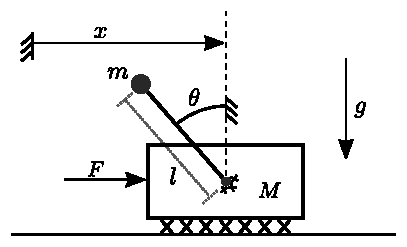
\includegraphics[width=.5\textwidth]{figures/mechanicalDrawing}\vspace{6pt}
  }  
\end{figure}


It is assumed that the pendulum rod is rigid and massless. This is deemed sensible, as the pendulum mass is much heavier than the hollow aluminum rod. The added inertia of the motor's rotor is also negligibly small, only \SI{54.2e-6}{kg\cdot m^2}, see \textit{Hardware} \autoref{sec:hardware}, compared to $ml = 0.201 \cdot 0.3348=$ \SI{67.3e-3}{kg\cdot m^2} contributed by the pendulum mass. The pendulum mass is modeled as a point mass placed at its geometrical center. This is why the length, $l$, is measured from the pivot point to the center of the pendulum mass.\\
The mass of the cart includes the weight of the belt and the wires hanging from the cart to the controller and supply. The influence of the wires will vary depending on the position of the cart, but this is treated as an unmodeled disturbance.\\
In the following two modeling approaches, fictions is represented as two unknown functions of generalized velocities, $\dot{x}$ and $\dot{\theta}$, denoted $B_c(\dot{x})$ for the cart and $B_p(\dot{\theta})$ for the pendulum. These functions are then modeled in \autoref{sec:frictionModel}.

\fxnote{review if all assumptions are included}



